\documentclass{article}

\usepackage{amsmath}
\usepackage{amssymb}
\usepackage[spanish]{babel}
\usepackage{cancel}
\usepackage[margin=1.5in]{geometry}
\usepackage{graphicx}
\usepackage[utf8]{inputenc}
\usepackage{tcolorbox}

\renewcommand{\Bbb}{\mathbb}

\tcbuselibrary{theorems}

\begin{document} 

\section{Teórica 1}

\subsection{El espacio vectorial $\Bbb R^n$}

El objetivo de la materia es adaptar los conceptos de Análisis I (derivadas, integrales, Taylor ...) al espacio n-dimensional, $\mathbb{R}^n$.

\begin{equation}
x \in \Bbb R^n \Longleftrightarrow x = (x_1, x_2, x_3, ..., x_n)
\end{equation}

Se dice que $x$ es un vector o punto de $\Bbb R^n$, compuesto por $n$ números reales. No se distingue entre vector y punto, salvo que sea necesario.

$\Bbb R^n$ se estructura en espacio vectorial definiendo las siguientes operaciones:

\begin{subequations}
\begin{align}
\forall x, y \in \Bbb R^n, & z = x + y \Longleftrightarrow z_i = x_i + y_i, \forall i \in [1, n] & \text{SUMA VECTORIAL}\\
\forall \alpha \in \Bbb R, & x \in \Bbb R^n, z = \alpha x \Longleftrightarrow z_i = \alpha x_i \forall i \in [1, n] & \text{PRODUCTO POR ESCALAR}
\end{align}
\end{subequations}

Con estas definiciones, puede probarse que $\Bbb R^n$ es cerrado para la suma vectorial y producto por un escalar, considerando el vector nulo (todos ceros), $\overline{0}$, como el neutro para la suma, y el número real 1 como el neutro del producto por escalar.

Adicionalmente, $\Bbb R^n$ pasa a ser un \textbf{espacio vectorial euclídeo} si se le agrega un \textbf{producto escalar}:

\begin{equation}
\forall x, y \in \Bbb R^n, \alpha = x \cdot y \Longleftrightarrow \alpha = \sum_{i=1}^{n} x_i y_i = x_1 y_1 + x_2 y_2 + ... + x_n y_n
\end{equation}

Definiendo una \textbf{norma} sobre el producto escalar, $\Bbb R^n$ pasa a ser un espacio vectorial euclídeo y normado. La norma canónica en $\Bbb R^n$ es la raíz cuadrada del producto escalar del vector consigo mismo:

\begin{equation}
\forall x \in \Bbb R^n, \|x\| = \sqrt{x \cdot x} = \sqrt{ \sum_{i=1}^{n} x_i^2 }
\end{equation}

Un \textbf{versor} es un vector de norma 1. Para "normalizar" cualquier vector, se lo divide por su norma:

\begin{equation}
\forall x \in \Bbb R^n, \left\| \frac{x}{\|x\|} \right\| = 1
\end{equation}

\subsection{Ángulo entre dos vectores - Proyección}

Si $x, y \neq \overline{0}$, el ángulo entre x e y, $\alpha(x,y)$, satisface la siguiente igualdad:

\begin{equation}
\cos (\alpha(x, y)) = \frac{x \cdot y}{ \|x\| \|y\| }
\end{equation}

\begin{figure}[t]
\caption{Proyección del vector x sobre el vector y}
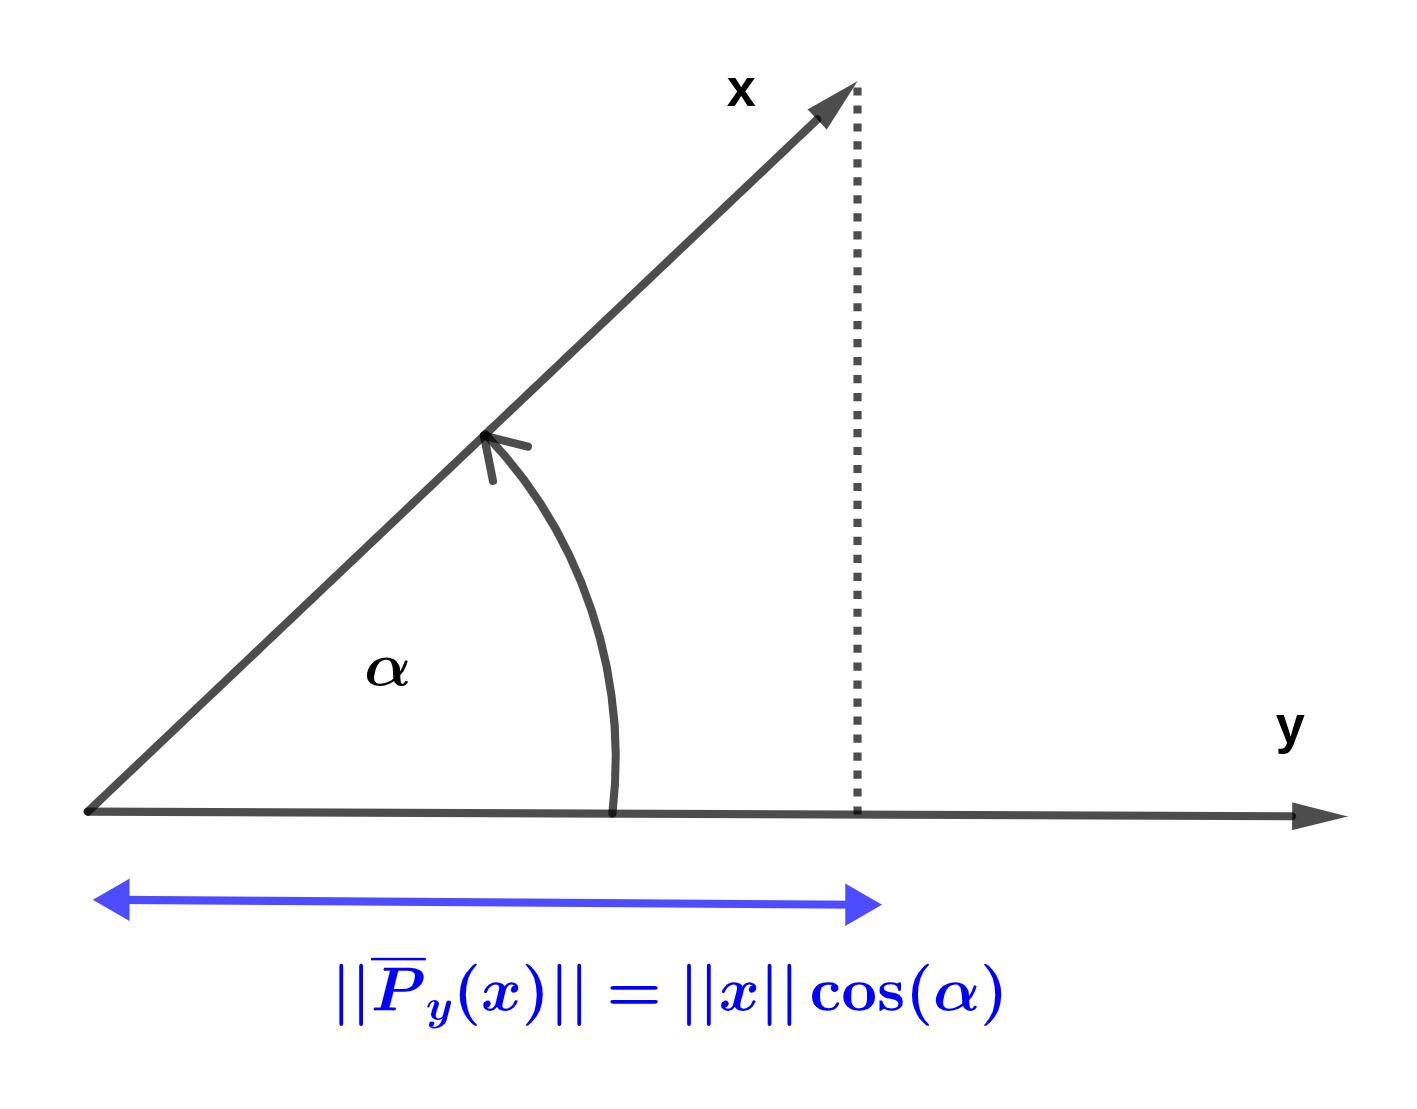
\includegraphics[scale=1]{img/teo_fig001_proyeccion.png} 
\centering
\label{fig:proyeccion}
\end{figure}

Aplicando la igualdad del ángulo entre vectores, y considerando el versor $\breve{y} = \frac{y}{\|y\|}$, resulta:

\begin{equation}
x \cdot y = \|x\| \|y\| \cos(\alpha) \Longrightarrow x \cdot \breve{y} = \|x\| \underbrace{ \cancel{ \| \breve{y} \| } }_{\text{Norma 1}} \cos(\alpha) = \|x\| \cos(\alpha)
\end{equation}

Geométricamente, como se observa en la figura ~\ref{fig:proyeccion}, la proyección de x sobre y se obtiene como el siguiente vector:

\begin{equation}
\overline{P}_{y}(x) =  \underbrace{ \|x\| \cos(\alpha) }_{\text{Escalar}}  \underbrace{ \breve{y} }_{\text{Versor}}
\end{equation}

\begin{equation}
\tcboxmath[colback=orange!25!white,colframe=orange, title=Proyección de x sobre y]
{ \overline{P}_{y}(x) = (x \cdot \breve{y}) \breve{y} }
\end{equation}

\begin{subequations}
\begin{align}
\overline{P}_{y}(x) = \overline{0} & \Longleftrightarrow x \perp y \Longleftrightarrow \cos \alpha = 0 \\
\overline{P}_{y}(x) = x & \Longleftrightarrow x = \alpha y, \alpha > 0
\end{align}
\end{subequations}

\subsection{Distancia entre dos puntos}

$\forall x, y \in \Bbb R^n$, se define la distancia entre x e y como:

\begin{equation}
d(x,y) = \| x - y \| = \| y - x \|
\end{equation}

\subsection{Producto vectorial}

Sólo para $\Bbb R^3$, se define el \textbf{producto vectorial} como:

\begin{equation}
\forall x, y \in \Bbb R^3: x \otimes y = \begin{vmatrix}
    \breve{i} & \breve{j} & \breve{k} \\
    x_1 & x_2 & x_3 \\ 
    y_1 & y_2 & y_3
  \end{vmatrix} =
\left(
  \begin{vmatrix} x_2 & x_3 \\ y_2 & y_3 \end{vmatrix},
  -\begin{vmatrix} x_1 & x_3 \\ y_1 & y_3 \end{vmatrix},
  \begin{vmatrix} x_1 & x_2 \\ y_1 & y_2 \end{vmatrix}
\right)
\end{equation}

Propiedades:

\begin{subequations}
\begin{align}
x \otimes y & \perp x \\
x \otimes y & \perp y \\
x \otimes y & = -y \otimes x \\
\| x \otimes y \| & = \|x\| \|y\| \sin(\alpha(x,y)) = \text{Área del paralelogramo determinado por x e y} \\
x \otimes y & = \overline{0} \Longleftrightarrow \{x, y\} \text{ es linealmente dependiente} \Longleftrightarrow x \parallel y
\end{align}
\end{subequations}

\subsection{Clasificación de puntos en un subconjunto de $\Bbb R^n$}

Sea un punto $P_0 \in \Bbb R^n$; se define como \textbf{bola o entorno} de centro $P_0$ y radio $r$ al conjunto de puntos cuya distancia a $P_0$ es menor que $r$. Simbólicamente:

\begin{equation}
B(P_0, r) = \{ x \in \Bbb R^n / \| x - P_0 \| < r \}
\end{equation}

En $\Bbb R$, esto es un intervalo abierto; en $\Bbb R^2$, el interior de un círculo; en $\Bbb R^3$, el interior de una esfera. Para dimensiones mayores, no hay tal representación geométrica, pero la definición se mantiene.

Si se excluye al centro $P_0$, se habla de una bola o entorno \textbf{reducido}:

\begin{equation}
B^*(P_0, r) = B(P_0, r) - \{ P_0 \}
\end{equation}

Considérese a continuación un subconjunto $A \subseteq \Bbb R^n$

\subsubsection{Punto interior}

$P_0$ es punto interior de $A \Longleftrightarrow \exists B(P_0, r) \subset A$. Es decir, si existe al menos un entorno centrado en $P_0$ que esté incluido en $A$. En otras palabras, $P_0$ está "rodeado por todas partes" de puntos de $A$.

Por otro lado, se define al \textbf{conjunto interior de} $A$, notado $\mathring{A}$, de la siguiente manera:

\begin{equation}
\mathring{A} = \{ x \in \Bbb R^n / x \text{ es punto interior de } A \}
\end{equation}

\subsubsection{Punto exterior}

$P_0$ es punto exterior de $A \Longleftrightarrow \exists B(P_0, r) \subset A^c$. Es decir, un punto es exterior de $A$ si es interior del complemento de $A$ ($A^c$).

\begin{equation}
Ext(A) = \{ x \in \Bbb R^n / x \text{ es p.e. de A } \}
\end{equation}

\subsubsection{Punto frontera}

$P_0$ es punto frontera de $A \Longleftrightarrow$ toda bola centrada en $P_0$ contiene elementos de $A$ y $A^c$. Simbólicamente:

\begin{equation}
P_0 \text{ es p.f. de } A \Longleftrightarrow \forall B(P_0, r), \left\{
\begin{array}{ll}
B(P_0, r) \cap A \neq \varnothing \\
B(P_0, r) \cap A^c \neq \varnothing
\end{array}
\right.
\end{equation}

La \textbf{frontera} de $A$, $\partial A$, se define como:

\begin{equation}
\partial A = \{ x \in \Bbb R^n / x \text{ es p.f. de A } \}
\end{equation}

Propiedades:

\begin{subequations}
\begin{align}
\mathring{A} \cap \partial A & = \varnothing \\
Ext(A) \cap \partial A & = \varnothing \\
\mathring{A} \cap Ext(A) & = \varnothing \\
\mathring{A} \cup \partial A \cup Ext(A) & = \Bbb R^n \\
\text{Clausura/adherencia de A } = \overline{A} & = A \cup \partial A \\
\text{A es abierto } \Longleftrightarrow A & = \mathring{A} \\
\text{A es cerrado } \Longleftrightarrow A & = \overline{A} \Longleftrightarrow A^c \text{ es abierto } \\
\end{align}
\end{subequations}

\subsubsection{Punto aislado}

$P_0$ es p.a. $\Longleftrightarrow \exists B^*(P_0, r) / B^*(P_0, r) \cap A = \varnothing$.

O sea, hay al menos un entorno reducido centrado en $P_0$ que no contiene otro elemento de $A$ aparte de $P_0$.

\subsubsection{Punto de acumulación}

$P_0$ es p. de ac. $\Longleftrightarrow \forall B^*(P_0, r), B^*(P_0, r) \cap A \neq \varnothing$.
Vale decir, en todo entorno reducido de $P_0$ hay elementos de $A$. El conjunto derivado de $A$, denotado $A'$, se define como el conjunto de todos los puntos de acumulación de $A: A' = \{ x \in \Bbb R^n / x \text{ x es p. de ac. de A} \}$

\end{document} 
